\documentclass{beamer}

\usepackage{amsmath,amsfonts}
\usepackage{bm}
\usepackage{nicefrac}
\usepackage{mathrsfs}
\usepackage{etex}
\usepackage{ccicons}
\usepackage{pgfplots,tikz}
\usepackage{tikz-qtree}
\usepackage{algorithms/algorithm}
\usepackage{algorithms/algorithmic}
\usepackage[T1]{fontenc}
\usepackage{cancel}
\usepackage{xcolor}
\usepackage{rotating}


\newlength\figureheight
\newlength\figurewidth

\definecolor{gray}{gray}{0.4}

\makeatletter
\@ifclassloaded{beamer}{
\usefonttheme[onlymath]{serif}
\uselanguage{French}
\languagepath{French}
% Git hash
\usepackage{xstring}
\usepackage{catchfile}
\immediate\write18{git rev-parse HEAD > git.hash}
\CatchFileDef{\HEAD}{git.hash}{\endlinechar=-1}
\newcommand{\gitrevision}{\StrLeft{\HEAD}{7}}
}{}
\makeatother

\makeatletter
\@ifclassloaded{beamer}{
\setbeamertemplate{footline}{
  {\hfill\vspace*{1pt}\href{https://creativecommons.org/publicdomain/zero/1.0/legalcode.en}{\ccZero}\hspace{.1cm}
    \href{https://mnemosyne.ithaca.fr/stephane/ep-mj-30-years/blob/\HEAD/tex/slides/sep.tex}{\gitrevision}\enspace--\enspace\today\enspace
  }}}
\makeatother

\makeatletter
\newenvironment{sqcases}{%
  \matrix@check\sqcases\env@sqcases
}{%
  \endarray\right.%
}
\def\env@sqcases{%
  \let\@ifnextchar\new@ifnextchar
  \left\lbrack
  \def\arraystretch{1.2}%
  \array{@{}l@{\quad}l@{}}%
}
\makeatother


\begin{document}

\setbeamertemplate{navigation symbols}{}


\title{The stochastic extended path approach}
\author{St\'ephane Adjemian\footnote{Universit\'e du Mans, Dynare team} and Michel Juillard\footnote{Dynare team}}
\date{February, 2025}

\begin{frame}
  \titlepage{}
\end{frame}


\begin{frame}
  \frametitle{Motivations}

  \begin{itemize}

  \item Nonlinearities can play an important role in macroeconomics:
    Irreversible investment, ZLB, Borrowing constraint, \ldots\newline

  \item Standard local approximation techniques fail to produce
    reliable results in the presence of kinks.\newline

  \item Deterministic, perfect forresight models can be solved with much
    greater accuracy than stochastic ones.\newline

  \item The extended path approach aims to leverage the accuracy of
    deterministic methods in capturing (deterministic) nonlinearities.\newline

  \item But it neglects the implications of future uncertainty. Is
    this a concern? Can we improve the EP approach?

  \end{itemize}
\end{frame}


\begin{frame}
\frametitle{Model to be solved}

\[
\mathbb E_t\left[ f\left( y_{t-1},y_t,y_{t+1},\varepsilon_t \right) \right] = 0
\]

\bigskip

\begin{itemize}

\item $y$ an $n\times 1$ vector of endogenous variables\newline

\item $f: \mathbb R^{3n+q}\rightarrow \mathbb R^n$\newline

\item $\varepsilon_t \sim \mathcal N\left( 0,\Sigma \right) \perp y_{\underline{t-1}}$\newline

\item $ \exists\, y^{\star}$ such that $f\left( y^{\star},y^{\star},y^{\star},0 \right)=0$

\end{itemize}

\end{frame}


\begin{frame}
  \frametitle{Perfect foresight version}

  \[
    \begin{cases}
      f\left( {\color{red}y_{t-1}},y_t,y_{t+1},\varepsilon_t \right) = 0\\
      f\left( y_{t+h-1},y_{t+h},y_{t+h+1}, 0 \right) = 0\quad \text{ for }h=1,\ldots,H-2\\
      f\left( y_{t+H-2},y_{t+H-1},{\color{red}y^{\star}}, 0 \right) = 0\\
    \end{cases}
  \]


  \begin{itemize}
  \item Perfect foresight models, after a shock economy returns asymptotically
    to equilibirum.
  \item For a long enough simulation, one can consider that for all
    practical purpose the system is back to equilibrium.
  \item This suggests to solve a two value boundary problem with
    initial conditions for some variables (backward looking) and
    terminal conditions for others (forward looking).
  \item In practice, one can use a Newton method to the equations of
    the model stacked over all periods of the simulation.
  \item The Jacobian matrix of the stacked system is very sparse and
    this characteristic must be used to write a practical algorithm.
  \end{itemize}

\end{frame}


\begin{frame}
  \frametitle{Solve perfect foresight models}
\end{frame}


\begin{frame}
  \frametitle{Stochastic perfect foresight models}
\end{frame}


\begin{frame}[c]{}
  \frametitle{Stochastic perfect foresight models}
  \framesubtitle{order 1}
  \centering
  \[
    \begin{split}
      &\sum_{i=1}^n\omega_i f\left( y_{i,t+1}, {\color{red} y_t}, {\color{blue} y_{t-1}}\right) = 0\\
      \begin{sideways}\hspace{-.6cm}\footnotesize{i=1,\dots,n}\end{sideways} &\begin{sqcases}
        f\left( y_{i,t+2}, y_{i,t+1}, {\color{red}y_t}, \epsilon_i \right) = 0\\
        f\left( y_{i,t+3}, y_{i,t+2}, y_{i,t+1}, 0 \right) = 0\\
        \vdots\\
        f\left( {\color{blue}y^{\star}}, y_{i,t+H-1}, y_{i,t+H-2}, 0 \right) = 0\\
      \end{sqcases}
    \end{split}
  \]

\end{frame}


\begin{frame}[c,fragile]{}
  \frametitle{Stochastic perfect foresight models}
  \framesubtitle{order 1}
  \centering

  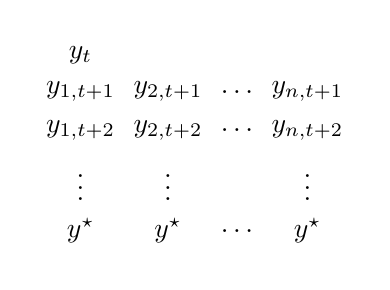
\begin{tikzpicture}
\matrix
  {
    \node {$y_t$}; & \node{}; & \node {}; & \node {}; \\
    \node {$y_{1,t+1}$}; & \node{$y_{2,t+1}$}; & \node{$\ldots$};& \node{$y_{n,t+1}$}; \\
    \node {$y_{1,t+2}$}; & \node{$y_{2,t+2}$}; & \node{$\ldots$};& \node{$y_{n,t+2}$}; \\
    \node {$\vdots$}; & \node{$\vdots$}; & \node{};& \node{$\vdots$}; \\
    \node {$y^\star$}; & \node{$y^\star$}; & \node{$\ldots$};& \node{$y^\star$}; \\
  };
\end{tikzpicture}

\end{frame}



\begin{frame}
  \frametitle{Stochastic perfect foresight model}
  \framesubtitle{Stacked jacobian, order=1, three nodes}
  \begin{center}
    \scalebox{.5}{
  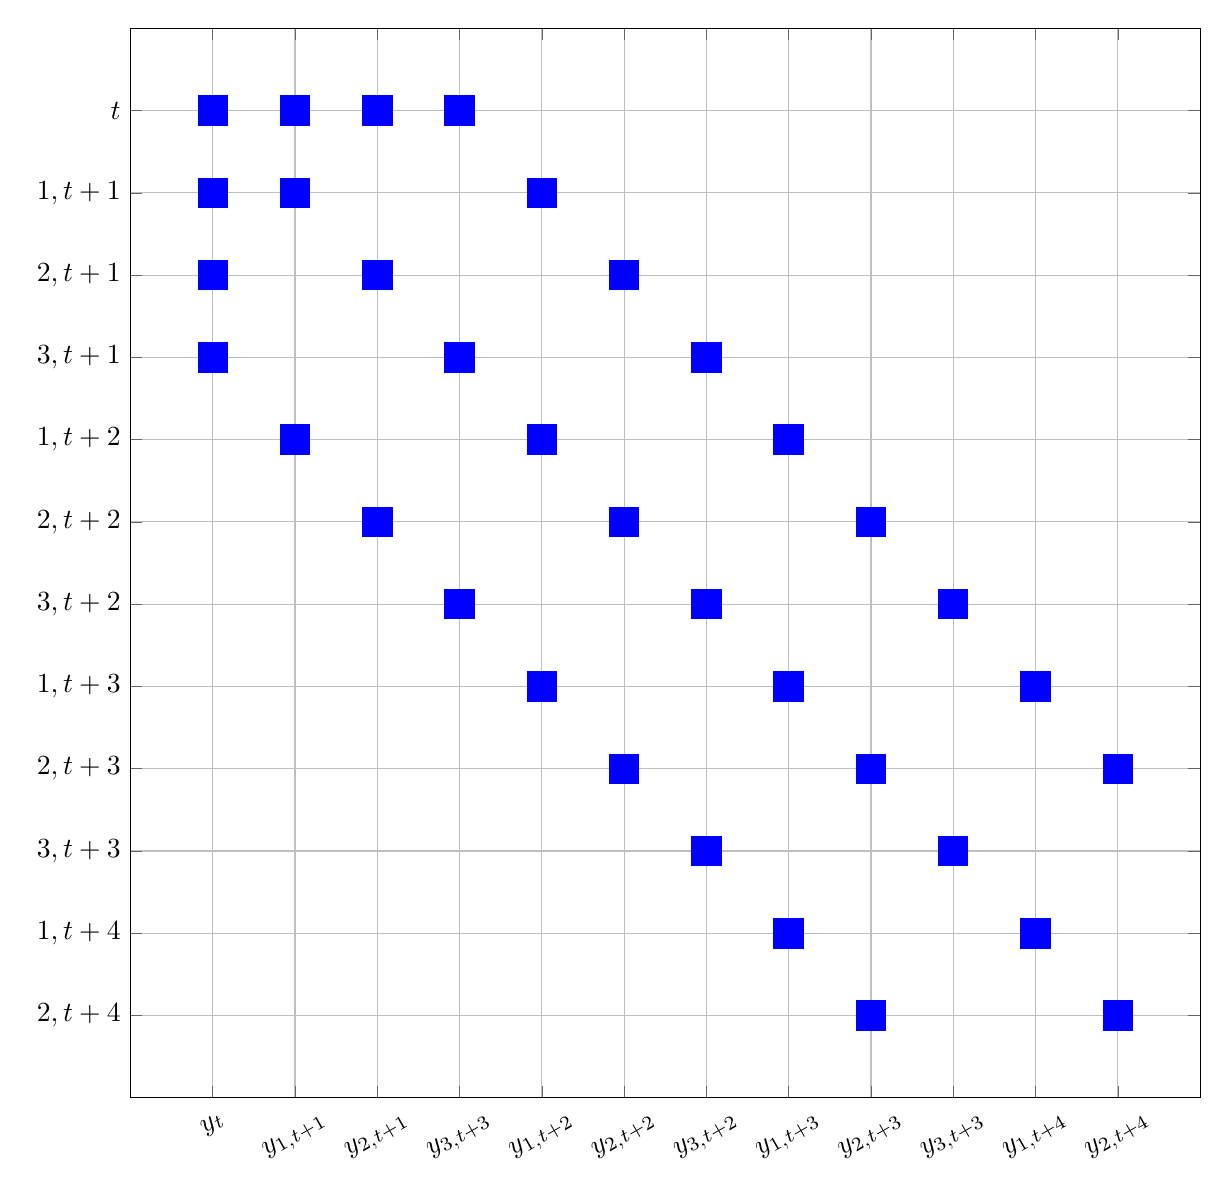
\begin{tikzpicture}

\begin{axis}[%
width=5.348in,
height=5.348in,
at={(1.854in,0.722in)},
scale only axis,
xmin=0,
xmax=13,
xtick={1,2,3,4,5,6,7,8,9,10,11,12},
xticklabels={$y_t$,$y_{1,t+1}$,$y_{2,t+1}$,$y_{3,t+3}$,$y_{1,t+2}$,$y_{2,t+2}$,$y_{3,t+2}$,$y_{1,t+3}$,$y_{2,t+3}$,$y_{3,t+3}$,$y_{1,t+4}$,$y_{2,t+4}$},
xticklabel style={rotate=30},
y dir=reverse,
ymin=0,
ymax=13,
ytick={1,2,3,4,5,6,7,8,9,10,11,12},
yticklabels={$t$,{$1,t+1$},{$2,t+1$},{$3,t+1$},{$1,t+2$},{$2,t+2$},{$3,t+2$},{$1,t+3$},{$2,t+3$},{$3,t+3$},{$1,t+4$},{$2,t+4$}},
axis background/.style={fill=white},
xmajorgrids,
ymajorgrids
]
\addplot [color=blue, only marks, mark size=5.3pt, mark=square*, mark options={solid, blue}, forget plot]
  table[row sep=crcr]
  \end{center}
\end{frame}


  \begin{frame}[c]{}
  \frametitle{Stochastic perfect foresight models}
  \framesubtitle{order 2}
  \centering

  \[
    \begin{split}
      &\sum_{i=1}^n\omega_i f\left( y_{i,t+1}, {\color{red} y_t}, {\color{blue} y_{t-1}}\right) = 0\\
      \begin{sideways}\hspace{-.6cm}\footnotesize{i=1,\dots,n}\end{sideways} & \begin{sqcases}
        \sum_{j=1}^n\omega_jf\left( y_{j,i,t+2}, y_{i,t+1}, {\color{red}y_t}, \epsilon_i \right) = 0\\
        \begin{sideways}\hspace{-.6cm}\footnotesize{j=1,\dots,n}\end{sideways} \begin{sqcases}
          f\left( y_{j,i,t+3}, y_{j,i,t+2}, y_{i,t+1}, \epsilon_j \right) = 0\\
          f\left( y_{j,i,t+4}, y_{j,i,t+3}, y_{j,i,t+2}, 0 \right) = 0\\
          \vdots\\
          f\left( {\color{blue}y^{\star}}, y_{j,i,t+H-1}, y_{j,i,t+H-2}, 0 \right) = 0
        \end{sqcases}
      \end{sqcases}
    \end{split}
  \]

  \end{frame}


  \begin{frame}[c,fragile]{}
  \frametitle{Stochastic perfect foresight models}
  \framesubtitle{order 2}
  \centering

  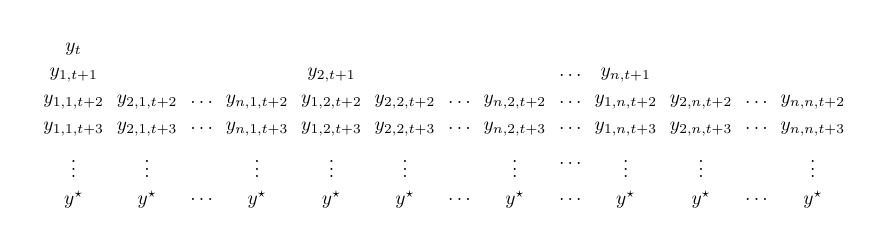
\begin{tikzpicture}[scale=0.6, every node/.style={scale=0.7}]
\matrix
  {
    \node {$y_t$}; & \node{}; & \node {}; & \node {}; \node {}; & \node{}; & \node {}; & \node {}; & \node{}; & \node{}; & \node {}; & \node {}; & \node{};\\
    \node {$y_{1,t+1}$}; & \node{}; & \node{}; & \node{}; & \node {$y_{2,t+1}$}; & \node{}; & \node{}; & \node{}; & \node{$\ldots$}; & \node {$y_{n,t+1}$}; & \node{}; & \node{}; & \node{}; \\
    \node {$y_{1,1,t+2}$}; & \node{$y_{2,1,t+2}$}; & \node{$\ldots$}; & \node{$y_{n,1,t+2}$}; & \node {$y_{1,2,t+2}$}; & \node{$y_{2,2,t+2}$}; & \node{$\ldots$}; & \node{$y_{n,2,t+2}$}; & \node{$\ldots$}; & \node {$y_{1,n,t+2}$}; & \node{$y_{2,n,t+2}$}; & \node{$\ldots$};& \node{$y_{n,n,t+2}$}; \\
    \node {$y_{1,1,t+3}$}; & \node{$y_{2,1,t+3}$}; & \node{$\ldots$}; & \node{$y_{n,1,t+3}$}; & \node {$y_{1,2,t+3}$}; & \node{$y_{2,2,t+3}$}; & \node{$\ldots$};& \node{$y_{n,2,t+3}$}; & \node{$\ldots$}; & \node {$y_{1,n,t+3}$}; & \node{$y_{2,n,t+3}$}; & \node{$\ldots$};& \node{$y_{n,n,t+3}$};\\
    \node {$\vdots$}; & \node{$\vdots$}; & \node{};& \node{$\vdots$}; & \node {$\vdots$}; & \node{$\vdots$}; & \node{};& \node{$\vdots$}; & \node{$\ldots$}; & \node {$\vdots$}; & \node{$\vdots$}; & \node{};& \node{$\vdots$};\\
    \node {$y^\star$}; & \node{$y^\star$}; & \node{$\ldots$};& \node{$y^\star$}; & \node {$y^\star$}; & \node{$y^\star$}; & \node{$\ldots$};& \node{$y^\star$}; & \node{$\ldots$}; & \node {$y^\star$}; & \node{$y^\star$}; & \node{$\ldots$};& \node{$y^\star$};\\
  };
\end{tikzpicture}

\end{frame}


  \begin{frame}
    \frametitle{Stochastic perfect foresight model}
    \framesubtitle{Stacked jacobian, order=2, three nodes}
  \begin{center}
    \scalebox{.5}{
  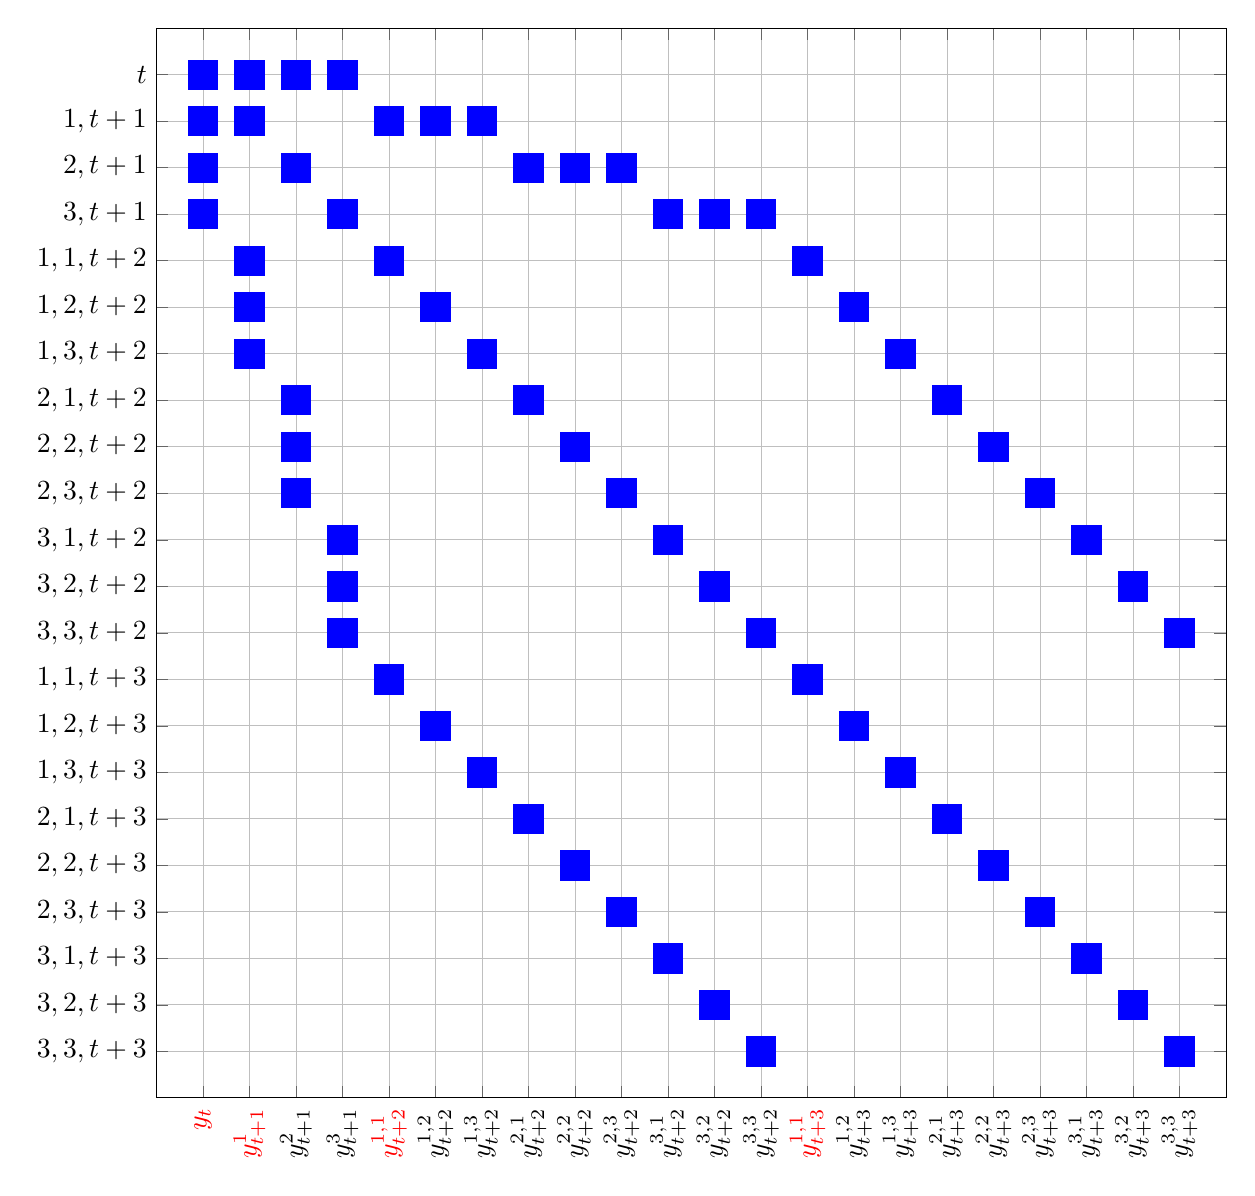
\begin{tikzpicture}

\begin{axis}[%
width=5.348in,
height=5.348in,
at={(1.854in,0.722in)},
scale only axis,
xmin=0,
xmax=23,
xtick={1,2,3,4,5,6,7,8,9,10,11,12,13,14,15,16,17,18,19,20,21,22},
xticklabels={{\color{red}$y_t$},{\color{red}$y_{t+1}^1$},{$y_{t+1}^2$},{$y_{t+1}^3$},{\color{red}$y_{t+2}^{1,1}$},{$y_{t+2}^{1,2}$},{$y_{t+2}^{1,3}$},{$y_{t+2}^{2,1}$},{$y_{t+2}^{2,2}$},{$y_{t+2}^{2,3}$},{$y_{t+2}^{3,1}$},{$y_{t+2}^{3,2}$},{$y_{t+2}^{3,3}$},{\color{red}$y_{t+3}^{1,1}$},{$y_{t+3}^{1,2}$},{$y_{t+3}^{1,3}$},{$y_{t+3}^{2,1}$},{$y_{t+3}^{2,2}$},{$y_{t+3}^{2,3}$},{$y_{t+3}^{3,1}$},{$y_{t+3}^{3,2}$},{$y_{t+3}^{3,3}$}},
xticklabel style={rotate=90},
y dir=reverse,
ymin=0,
ymax=23,
ytick={1,2,3,4,5,6,7,8,9,10,11,12,13,14,15,16,17,18,19,20,21,22},
yticklabels={$t$,{$1,t+1$},{$2,t+1$},{$3,t+1$},{$1,1,t+2$},{$1,2,t+2$},{$1,3,t+2$},{$2,1,t+2$},{$2,2,t+2$},{$2,3,t+2$},{$3,1,t+2$},{$3,2,t+2$},{$3,3,t+2$},{$1,1,t+3$},{$1,2,t+3$},{$1,3,t+3$},{$2,1,t+3$},{$2,2,t+3$},{$2,3,t+3$},{$3,1,t+3$},{$3,2,t+3$},{$3,3,t+3$}},
axis background/.style={fill=white},
xmajorgrids,
ymajorgrids
]
\addplot [color=blue, only marks, mark size=5.3pt, mark=square*, mark options={solid, blue}, forget plot]
  table[row sep=crcr]
  \end{center}

\end{frame}


\end{document}
